% -*- Mode:TeX -*-

%% IMPORTANT: The official thesis specifications are available at:
%%            http://libraries.mit.edu/archives/thesis-specs/
%%
%%            Please verify your thesis' formatting and copyright
%%            assignment before submission.  If you notice any
%%            discrepancies between these templates and the 
%%            MIT Libraries' specs, please let us know
%%            by e-mailing thesis@mit.edu

%% The documentclass options along with the pagestyle can be used to generate
%% a technical report, a draft copy, or a regular thesis.  You may need to
%% re-specify the pagestyle after you \include  cover.tex.  For more
%% information, see the first few lines of mitthesis.cls. 

%\documentclass[12pt,vi,twoside]{mitthesis}
%%
%%  If you want your thesis copyright to you instead of MIT, use the
%%  ``vi'' option, as above.
%%
%\documentclass[12pt,twoside,leftblank]{mitthesis}
%%
%% If you want blank pages before new chapters to be labelled ``This
%% Page Intentionally Left Blank'', use the ``leftblank'' option, as
%% above. 

\documentclass[12pt,twoside]{mitthesis}
\usepackage{lgrind}
%% These have been added at the request of the MIT Libraries, because
%% some PDF conversions mess up the ligatures.  -LB, 1/22/2014
\usepackage{cmap}
\usepackage[T1]{fontenc}
\pagestyle{plain}

%% This bit allows you to either specify only the files which you wish to
%% process, or `all' to process all files which you \include.
%% Krishna Sethuraman (1990).

\typein [\files]{Enter file names to process, (chap1,chap2 ...), or `all' to
process all files:}
\def\all{all}
\ifx\files\all \typeout{Including all files.} \else \typeout{Including only \files.} \includeonly{\files} \fi

\begin{document}

% -*-latex-*-
% 
% For questions, comments, concerns or complaints:
% thesis@mit.edu
% 
%
% $Log: cover.tex,v $
% Revision 1.8  2008/05/13 15:02:15  jdreed
% Degree month is June, not May.  Added note about prevdegrees.
% Arthur Smith's title updated
%
% Revision 1.7  2001/02/08 18:53:16  boojum
% changed some \newpages to \cleardoublepages
%
% Revision 1.6  1999/10/21 14:49:31  boojum
% changed comment referring to documentstyle
%
% Revision 1.5  1999/10/21 14:39:04  boojum
% *** empty log message ***
%
% Revision 1.4  1997/04/18  17:54:10  othomas
% added page numbers on abstract and cover, and made 1 abstract
% page the default rather than 2.  (anne hunter tells me this
% is the new institute standard.)
%
% Revision 1.4  1997/04/18  17:54:10  othomas
% added page numbers on abstract and cover, and made 1 abstract
% page the default rather than 2.  (anne hunter tells me this
% is the new institute standard.)
%
% Revision 1.3  93/05/17  17:06:29  starflt
% Added acknowledgements section (suggested by tompalka)
% 
% Revision 1.2  92/04/22  13:13:13  epeisach
% Fixes for 1991 course 6 requirements
% Phrase "and to grant others the right to do so" has been added to 
% permission clause
% Second copy of abstract is not counted as separate pages so numbering works
% out
% 
% Revision 1.1  92/04/22  13:08:20  epeisach

% NOTE:
% These templates make an effort to conform to the MIT Thesis specifications,
% however the specifications can change.  We recommend that you verify the
% layout of your title page with your thesis advisor and/or the MIT 
% Libraries before printing your final copy.
\title{Reading Between the (Party) Lines: \\ \emph{An Analysis of Media Trust}}

\author{Sophie Beiying Chou}
% If you wish to list your previous degrees on the cover page, use the 
% previous degrees command:
%       \prevdegrees{A.A., Harvard University (1985)}
% You can use the \\ command to list multiple previous degrees
%       \prevdegrees{B.S., University of California (1978) \\
%                    S.M., Massachusetts Institute of Technology (1981)}
\department{MIT Media Lab}
\school{School of Architecture and Planning}

% If the thesis is for two degrees simultaneously, list them both
% separated by \and like this:
% \degree{Doctor of Philosophy \and Master of Science}
\degree{MS in Media Arts and Sciences}

% As of the 2007-08 academic year, valid degree months are September, 
% February, or June.  The default is June.
\degreemonth{June}
\degreeyear{2016}
\thesisdate{May 5, 2016}

%% By default, the thesis will be copyrighted to MIT.  If you need to copyright
%% the thesis to yourself, just specify the `vi' documentclass option.  If for
%% some reason you want to exactly specify the copyright notice text, you can
%% use the \copyrightnoticetext command.  
%\copyrightnoticetext{\copyright IBM, 1990.  Do not open till Xmas.}

% If there is more than one supervisor, use the \supervisor command
% once for each.
\supervisor{Deb Roy}{Associate Professor}

% This is the department committee chairman, not the thesis committee
% chairman.  You should replace this with your Department's Committee
% Chairman. 
\chairman{Pattie Maes}{Academic Head, Program in Media Arts and Sciences}

% Make the titlepage based on the above information.  If you need
% something special and can't use the standard form, you can specify
% the exact text of the titlepage yourself.  Put it in a titlepage
% environment and leave blank lines where you want vertical space.
% The spaces will be adjusted to fill the entire page.  The dotted
% lines for the signatures are made with the \signature command.
\maketitle

% The abstractpage environment sets up everything on the page except
% the text itself.  The title and other header material are put at the
% top of the page, and the supervisors are listed at the bottom.  A
% new page is begun both before and after.  Of course, an abstract may
% be more than one page itself.  If you need more control over the
% format of the page, you can use the abstract environment, which puts
% the word "Abstract" at the beginning and single spaces its text.

%% You can either \input (*not* \include) your abstract file, or you can put
%% the text of the abstract directly between the \begin{abstractpage} and
%% \end{abstractpage} commands.

% First copy: start a new page, and save the page number.
\cleardoublepage
% Uncomment the next line if you do NOT want a page number on your
% abstract and acknowledgments pages.
% \pagestyle{empty}
\setcounter{savepage}{\thepage}
\begin{abstractpage}
% this environment should probably be called abstract,
% but we want people to also be able to get at the more
% basic abstract environment
\def\abstractpage{\cleardoublepage
\begin{center}{\large{\bf \@title} \\
by \\
\@author \\[\baselineskip]}
\par
\def\baselinestretch{1}\@normalsize
Submitted to the \@department, \\
\@school \\
on \@thesisdate, in partial fulfillment of the \\
requirements for the \@degreeword\ of \\
\@degree
\end{center}
\par
\begin{abstract}}

TO-DO
\end{abstractpage}

% Additional copy: start a new page, and reset the page number.  This way,
% the second copy of the abstract is not counted as separate pages.
% Uncomment the next 6 lines if you need two copies of the abstract
% page.
% \setcounter{page}{\thesavepage}
% \begin{abstractpage}
% % this environment should probably be called abstract,
% but we want people to also be able to get at the more
% basic abstract environment
\def\abstractpage{\cleardoublepage
\begin{center}{\large{\bf \@title} \\
by \\
\@author \\[\baselineskip]}
\par
\def\baselinestretch{1}\@normalsize
Submitted to the \@department, \\
\@school \\
on \@thesisdate, in partial fulfillment of the \\
requirements for the \@degreeword\ of \\
\@degree
\end{center}
\par
\begin{abstract}}

TO-DO
% \end{abstractpage}

 

%%%%%%%%%%%%%%%%%%%%%%%%%%%%%%%%%%%%%%%%%%%%%%%%%%%%%%%%%%%%%%%%%%%%%%
% -*-latex-*-

% Some departments (e.g. 5) require an additional signature page.  See
% signature.tex for more information and uncomment the following line if
% applicable.
% % -*- Mode:TeX -*-
%
% Some departments (e.g. Chemistry) require an additional cover page
% with signatures of the thesis committee.  Please check with your
% thesis advisor or other appropriate person to determine if such a 
% page is required for your thesis.  
%
% If you choose not to use the "titlepage" environment, a \newpage
% commands, and several \vspace{\fill} commands may be necessary to
% achieve the required spacing.  The \signature command is defined in
% the "mitthesis" class
%
% The following sample appears courtesy of Ben Kaduk <kaduk@mit.edu> and
% was used in his June 2012 doctoral thesis in Chemistry. 

\begin{titlepage}
\begin{large}
The following people served as readers for this thesis:

\signature{Sepandar Kamvar}{Associate Professor of Media Arts and Sciences \\
   MIT Media Lab}

\signature{Iyad Rahwan}{Associate Professor of Media Arts and Sciences \\
   MIT Media Lab}
 
\end{large}
\end{titlepage}
 
\cleardoublepage

\section*{Acknowledgments}

Thank you famiry-- sister
Thank you Linda and Keira
Thank you Deb
Thank you Ethan
THANK YOU NATHAN, I DON'T KNOW HOW YOU DO IT ALL
Thank you readers
Thank you LSM
Thank you Heather
Thank you figure makers 
Thank you Ramesh



\pagestyle{plain}
  % -*- Mode:TeX -*-
%% This file simply contains the commands that actually generate the table of
%% contents and lists of figures and tables.  You can omit any or all of
%% these files by simply taking out the appropriate command.  For more
%% information on these files, see appendix C.3.3 of the LaTeX manual. 
\tableofcontents
%\newpage 
\afterpage{\blankpage}
%\listoffigures
%\newpage
%\listoftables


%% This is an example first chapter.  You should put chapter/appendix that you
%% write into a separate file, and add a line \include{yourfilename} to
%% main.tex, where `yourfilename.tex' is the name of the chapter/appendix file.
%% You can process specific files by typing their names in at the 
%% \files=
%% prompt when you run the file main.tex through LaTeX.

\chapter{Introduction} 

Does anyone trust the news anymore? Not according to the latest Gallup Poll, which showed that only 4 in 10 Americans believe that mass media does a good job of reporting the news ``fully, fairly, and accurately.'' It's a major decline since the survey was first taken in 1999, back when more than half (55\%) of Americans believed the news was trustworthy.

And the trend has been steadily downward: in short, the majority of Americans have had little to no trust in mass media news coverage since 2007: a discouraging view for a tumultuous time in journalism \cite{Gallup-trust-2015}.

But beyond frustrated readers and reporters, why does distrust in the news matter? For one, media bias---or at the very least, the \emph{belief of} a biased media bias---may have a significant impact on the practice of democracy. A 2006 study from Georgetown University shows that those with more negative attitudes towards the news tend to be more highly influenced by their partisan prior beliefs and less by contemporary issues and messages when voting \cite{ladd2005attitudes}. This implies that distrust of media plays a potential role in the polarization of American politics.

Additionally, our reactions to news stories-- as well as politics at large-- are largely driven by emotion. Historical trends, as well as present-day models, show a process largely influenced by feelings rather than facts.


In light of the upcoming 2016 elections, Part I explores perceptions of media trust in coverage of the presidential candidates. Claims of media bias and favoritism are especially high-stakes in election years, where trust has been shown to plummet \cite{Gallup-trust-2015}.  

We begin by examining some of the factors that contribute to the perception of media bias. In particular, how does the \emph{content} of a story (reading level and vocabulary) affect the reader versus the \emph{context} (source)? Although studies have been conducted to both examine the psychological effect of wording on believability and the impact of media brands and bias, separating and comparing these two factors remains largely unexamined \cite{weisberg2008seductive, baum2008eye}

To test our hypotheses on news trust, we perform a study on the crowdsourcing platform CrowdFlower. We manipulate the source of the story to examine effects of media brands on the reader, and also compare trust rankings between high and low reading level stories.


% From our findings in an experimental setting, we then extrapolate to another dimension of media: the social sphere of Twitter. In this dimension, we look for emotional signals in the text that cause it to become universally popular, with the goal of finding patterns cross party divides.

Although the general consensus of mistrust is clear, perception of media bias is a complex phenomenon to dissect, as it combines social and psychological effects with the traits of the story itself. This section hopes to shed light on some of these factors.

% This thesis hopes to shed new light on understanding what motivates readers' trust and distrust of news media, and pave pathways to understanding virality in the political news media. 
%  
\chapter{The Power of (Percieved) Media Bias}




\section{The Effects of Media Bias}

%Why is media bias IMPORTANT? Why is the problem IMPORTANT?

 
%- Fox News Effect
%- Does the media matter


\section{The Role of the Reader in Perceptions of Bias}

It comes as no surprise that our own political stances have a significant effect in our perceptions of bias in the media. 

In even seemingly neutral stories, partisans tend to view reporting as biased against their own views. This phenomenon---deemed the ``hostile media effect''---was first studied at Stanford University by Robert P. Vallone, Lee Ross, and Mark R. Lepper in 1985 \cite{vallone1985hostile}. Although ``true'' neutrality of a story is nearly impossible to quantify due to the subjective nature of the concept, Vallone et. al were able to successfully demonstrate that partisans of \emph{both} sides (pro-Israeli and pro-Arab) viewed the same news segments as hostile towards their beliefs and favorable to the other side.

%? Perceptions of media bias, then, have as much to do as self-serving motivations to secure preferential treatment as they do with the media itself.
  
%? The political leanings of the reader are essential considerations when attempting to measure other factors that contribute to bias. In 

\section{The Role of Media Brands in Perceptions of Bias}
%The media, of course, is not just one unified mass, and in an increasingly fragmented ecosystem, the role of media brands is a crucial factor in the perception of bias. Although most research
%\cite{baum2008eye}


 
%For instance, most research on the hostile media phenomenon conceptualizes the news media as an undifferentiated mass of information sources that individuals can (and do) reasonably characterize as having a uniform political orientation (Giner-Sorolla and Chaiken 1994, Peffley et al. 2001, Eveland and Shah 2003). Yet, the past two decades have seen a dramatic increase in the number and variety of news sources. One consequence is that Democrats and Republicans are increasingly likely to differ systematically in their assessments of specific media outlets.






%With the decline of print newspapers, a diverse number of new platforms and web-centric publications have risen.


%How do you control for the above things in your study?

\section{The Role of Language [Policial Persuasion]}




\subsection{Language and Politics}
%Presidential speeches degrading over time-- ie simple language appeals to the masses in politics
\subsection{The Seductive Allure [... of Simple] Language}
%But we trust complex language for explaining technical facts

%Test image

%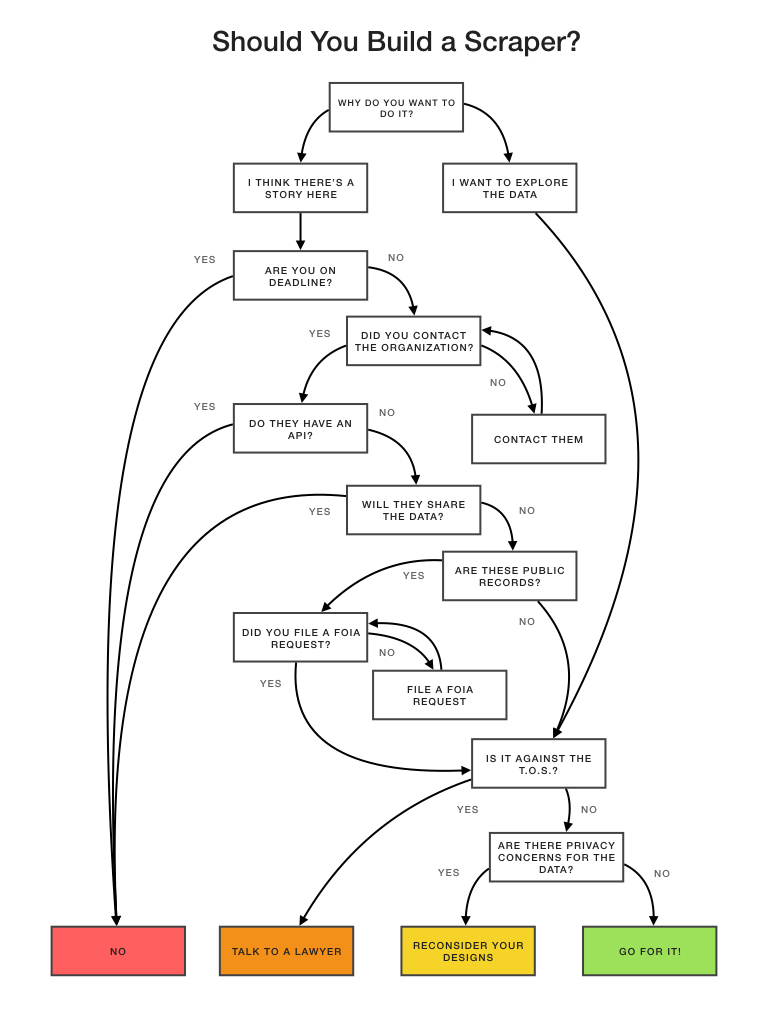
\includegraphics[width=\textwidth]{flowchart_final}


\section{Importance in Political Outcomes}
%Fox news effect 

\section{The 2016 Elections} 
\subsection{Criticism of Media Bias} 
%(Obama Speech)

%So.... are you what you cover?









\appendix
\chapter{Tables}
 %%%%%%%%%%%%%%%%%%%%% The unaffiliated %%%%%%%%%%%%%%%%%%%%%%%%%%%%%%%%%
\begin{table}[!htbp] \centering 
  \caption{Tweet Volume vs. Story Length, the Unaffiliated} 
  \label{} 
    \begin{tabular}{@{\extracolsep{5pt}}lccc} 
    \\[-1.8ex]\hline 
    \hline \\[-1.8ex] 
     & \multicolumn{3}{c}{\textit{Dependent variable:}} \\ 
    \cline{2-4} 
    \\[-1.8ex] & \multicolumn{3}{c}{Number of Tweets} \\ 
    \\[-1.8ex] & \textit{OLS} & \textit{Poisson} & \textit{negative} \\ 
     & \textit{} & \textit{} & \textit{binomial} \\ 
    \\[-1.8ex] & (1) & (2) & (3)\\ 
    \hline \\[-1.8ex] 
     Story length & $-$0.008$^{***}$ & $-$0.0004$^{***}$ & $-$0.0003$^{***}$ \\ 
      & (0.001) & (0.00001) & (0.00002) \\ 
      & & & \\ 
     Constant & 35.299$^{***}$ & 3.683$^{***}$ & 3.605$^{***}$ \\ 
      & (1.168) & (0.006) & (0.031) \\ 
      & & & \\ 
    \hline \\[-1.8ex] 
    Observations$^{*}$ & 2,640 & 2,640 & 2,640 \\ 
    R$^{2}$ & 0.029 &  &  \\ 
    Adjusted R$^{2}$ & 0.028 &  &  \\ 
    Log Likelihood &  & $-$49,432.820 & $-$11,415.510 \\ 
    $\theta$ &  &  & 0.954$^{***}$  (0.024) \\ 
    Akaike Inf. Crit. &  & 98,869.640 & 22,835.020 \\ 
    Residual Std. Error & 38.604 (df = 2638) &  &  \\ 
    F Statistic & 77.414$^{***}$ (df = 1; 2638) &  &  \\ 
    \hline 
    \hline \\[-1.8ex] 
    \textit{Note:}  & \multicolumn{3}{r}{$^{*}$p$<$0.1; $^{**}$p$<$0.05; $^{***}$p$<$0.01;} \\  
    \end{tabular}   
\end{table} 
\emph{$^{*}$We exclude stories not shared by this segment.}  
\newpage 
% Table created by stargazer v.5.2 by Marek Hlavac, Harvard University. E-mail: hlavac at fas.harvard.edu
% Date and time: Sun, Jul 24, 2016 - 19:08:45
\begin{table}[!htbp] \centering 
  \caption{Tweet Volume vs. Emotionality, the Unaffiliated} 
      \label{} 
    \begin{tabular}{@{\extracolsep{5pt}}lccc} 
    \\[-1.8ex]\hline 
    \hline \\[-1.8ex] 
     & \multicolumn{3}{c}{\textit{Dependent variable:}} \\ 
    \cline{2-4} 
    \\[-1.8ex] & \multicolumn{3}{c}{Number of Tweets} \\ 
    \\[-1.8ex] & \textit{OLS} & \textit{Poisson} & \textit{negative} \\ 
     & \textit{} & \textit{} & \textit{binomial} \\ 
    \\[-1.8ex] & (1) & (2) & (3)\\ 
    \hline \\[-1.8ex] 
     Emotionality & 248.768$^{***}$ & 8.165$^{***}$ & 7.427$^{***}$ \\ 
      & (79.579) & (0.347) & (2.145) \\ 
      & & & \\ 
     Constant & 22.519$^{***}$ & 3.147$^{***}$ & 3.162$^{***}$ \\ 
      & (1.747) & (0.008) & (0.047) \\ 
      & & & \\ 
    \hline \\[-1.8ex] 
    Observations$^{*}$ & 2,640 & 2,640 & 2,640 \\ 
    R$^{2}$ & 0.004 &  &  \\ 
    Adjusted R$^{2}$ & 0.003 &  &  \\ 
    Log Likelihood &  & $-$51,967.750 & $-$11,419.630 \\ 
    $\theta$ &  &  & 0.928$^{***}$  (0.023) \\ 
    Akaike Inf. Crit. &  & 103,939.500 & 22,843.260 \\ 
    Residual Std. Error & 39.094 (df = 2638) &  &  \\ 
    F Statistic & 9.772$^{***}$ (df = 1; 2638) &  &  \\ 
    \hline 
    \hline \\[-1.8ex] 
    \textit{Note:}  & \multicolumn{3}{r}{$^{*}$p$<$0.1; $^{**}$p$<$0.05; $^{***}$p$<$0.01} \\ 
    \end{tabular} 
\end{table}
\emph{$^{*}$We exclude stories not shared by this segment.}  
\newpage 
% Table created by stargazer v.5.2 by Marek Hlavac, Harvard University. E-mail: hlavac at fas.harvard.edu
% Date and time: Sun, Jul 24, 2016 - 19:09:28
\begin{table}[!htbp] \centering 
  \caption{Tweet Volume vs. Positivity, the Unaffiliated} 
  \label{} 
    \begin{tabular}{@{\extracolsep{5pt}}lccc} 
    \\[-1.8ex]\hline 
    \hline \\[-1.8ex] 
     & \multicolumn{3}{c}{\textit{Dependent variable:}} \\ 
    \cline{2-4} 
    \\[-1.8ex] & \multicolumn{3}{c}{Number of Tweets} \\ 
    \\[-1.8ex] & \textit{OLS} & \textit{Poisson} & \textit{negative} \\ 
     & \textit{} & \textit{} & \textit{binomial} \\ 
    \\[-1.8ex] & (1) & (2) & (3)\\ 
    \hline \\[-1.8ex] 
     Positivity & $-$145.324 & $-$5.277$^{***}$ & $-$4.036$^{*}$ \\ 
      & (90.790) & (0.440) & (2.452) \\ 
      & & & \\ 
     Constant & 27.797$^{***}$ & 3.324$^{***}$ & 3.321$^{***}$ \\ 
      & (0.795) & (0.004) & (0.021) \\ 
      & & & \\ 
    \hline \\[-1.8ex] 
    Observations$^{*}$ & 2,640 & 2,640 & 2,640 \\ 
    R$^{2}$ & 0.001 &  &  \\ 
    Adjusted R$^{2}$ & 0.001 &  &  \\ 
    Log Likelihood &  & $-$52,150.640 & $-$11,424.900 \\ 
    $\theta$ &  &  & 0.925$^{***}$  (0.023) \\ 
    Akaike Inf. Crit. &  & 104,305.300 & 22,853.790 \\ 
    Residual Std. Error & 39.147 (df = 2638) &  &  \\ 
    F Statistic & 2.562 (df = 1; 2638) &  &  \\ 
    \hline 
    \hline \\[-1.8ex] 
    \textit{Note:}  & \multicolumn{3}{r}{$^{*}$p$<$0.1; $^{**}$p$<$0.05; $^{***}$p$<$0.01} \\ 
    \end{tabular} 
\end{table}
\emph{$^{*}$We exclude stories not shared by this segment.} 
\newpage 

 %%%%%%%%%%%%%%%%%%% Single Candid %%%%%%%%%%%%%%%%%%%%%%%%%%%%%%%%%
% Table created by stargazer v.5.2 by Marek Hlavac, Harvard University. E-mail: hlavac at fas.harvard.edu
% Date and time: Sun, Jul 24, 2016 - 19:18:20
\begin{table}[!htbp] \centering 
  \caption{Tweet Volume vs. Story Length, Single-Candidate Followers} 
  \label{} 
    \begin{tabular}{@{\extracolsep{5pt}}lccc} 
    \\[-1.8ex]\hline 
    \hline \\[-1.8ex] 
     & \multicolumn{3}{c}{\textit{Dependent variable:}} \\ 
    \cline{2-4} 
    \\[-1.8ex] & \multicolumn{3}{c}{Number of Tweets} \\ 
    \\[-1.8ex] & \textit{OLS} & \textit{Poisson} & \textit{negative} \\ 
     & \textit{} & \textit{} & \textit{binomial} \\ 
    \\[-1.8ex] & (1) & (2) & (3)\\ 
    \hline \\[-1.8ex] 
     Story length & 0.002$^{***}$ & 0.0001$^{***}$ & 0.0002$^{***}$ \\ 
      & (0.0004) & (0.00001) & (0.00002) \\ 
      & & & \\ 
     Constant & 7.979$^{***}$ & 2.135$^{***}$ & 2.080$^{***}$ \\ 
      & (0.467) & (0.009) & (0.028) \\ 
      & & & \\ 
    \hline \\[-1.8ex] 
    Observations$^{*}$ & 2,581 & 2,581 & 2,581 \\ 
    R$^{2}$ & 0.007 &  &  \\ 
    Adjusted R$^{2}$ & 0.006 &  &  \\ 
    Log Likelihood &  & $-$17,969.510 & $-$8,449.973 \\ 
    $\theta$ &  &  & 1.330$^{***}$  (0.039) \\ 
    Akaike Inf. Crit. &  & 35,943.020 & 16,903.950 \\ 
    Residual Std. Error & 15.242 (df = 2579) &  &  \\ 
    F Statistic & 17.223$^{***}$ (df = 1; 2579) &  &  \\ 
    \hline 
    \hline \\[-1.8ex] 
    \textit{Note:}  & \multicolumn{3}{r}{$^{*}$p$<$0.1; $^{**}$p$<$0.05; $^{***}$p$<$0.01} \\ 
    \end{tabular} 
\end{table}
\emph{$^{*}$We exclude stories not shared by this segment.} 
\newpage 
% Table created by stargazer v.5.2 by Marek Hlavac, Harvard University. E-mail: hlavac at fas.harvard.edu
% Date and time: Sun, Jul 24, 2016 - 19:18:51
\begin{table}[!htbp] \centering 
  \caption{Tweet Volume vs. Emotionality, Single-Candidate Followers} 
  \label{} 
    \begin{tabular}{@{\extracolsep{5pt}}lccc} 
    \\[-1.8ex]\hline 
    \hline \\[-1.8ex] 
     & \multicolumn{3}{c}{\textit{Dependent variable:}} \\ 
    \cline{2-4} 
    \\[-1.8ex] & \multicolumn{3}{c}{Number of Tweets} \\ 
    \\[-1.8ex] & \textit{OLS} & \textit{Poisson} & \textit{negative} \\ 
     & \textit{} & \textit{} & \textit{binomial} \\ 
    \\[-1.8ex] & (1) & (2) & (3)\\ 
    \hline \\[-1.8ex] 
     Emotionality & 41.896 & 4.211$^{***}$ & 4.821$^{**}$ \\ 
      & (31.596) & (0.638) & (1.917) \\ 
      & & & \\ 
     Constant & 8.640$^{***}$ & 2.164$^{***}$ & 2.152$^{***}$ \\ 
      & (0.691) & (0.014) & (0.042) \\ 
      & & & \\ 
    \hline \\[-1.8ex] 
    Observations$^{*}$ & 2,581 & 2,581 & 2,581 \\ 
    R$^{2}$ & 0.001 &  &  \\ 
    Adjusted R$^{2}$ & 0.0003 &  &  \\ 
    Log Likelihood &  & $-$18,113.130 & $-$8,470.986 \\ 
    $\theta$ &  &  & 1.309$^{***}$  (0.038) \\ 
    Akaike Inf. Crit. &  & 36,230.260 & 16,945.970 \\ 
    Residual Std. Error & 15.288 (df = 2579) &  &  \\ 
    F Statistic & 1.758 (df = 1; 2579) &  &  \\ 
    \hline 
    \hline \\[-1.8ex] 
    \textit{Note:}  & \multicolumn{3}{r}{$^{*}$p$<$0.1; $^{**}$p$<$0.05; $^{***}$p$<$0.01} \\ 
    \end{tabular} 
\end{table}
\emph{$^{*}$We exclude stories not shared by this segment.}  
\newpage 
% Table created by stargazer v.5.2 by Marek Hlavac, Harvard University. E-mail: hlavac at fas.harvard.edu
% Date and time: Sun, Jul 24, 2016 - 19:20:38
\begin{table}[!htbp] \centering 
  \caption{Tweet Volume vs. Positivity, Single-Candidate Followers} 
  \label{} 
    \begin{tabular}{@{\extracolsep{5pt}}lccc} 
    \\[-1.8ex]\hline 
    \hline \\[-1.8ex] 
     & \multicolumn{3}{c}{\textit{Dependent variable:}} \\ 
    \cline{2-4} 
    \\[-1.8ex] & \multicolumn{3}{c}{Number of Tweets} \\ 
    \\[-1.8ex] & \textit{OLS} & \textit{Poisson} & \textit{negative} \\ 
     & \textit{} & \textit{} & \textit{binomial} \\ 
    \\[-1.8ex] & (1) & (2) & (3)\\ 
    \hline \\[-1.8ex] 
     Positivity & $-$70.477$^{*}$ & $-$7.387$^{***}$ & $-$8.385$^{***}$ \\ 
      & (36.056) & (0.758) & (2.202) \\ 
      & & & \\ 
     Constant & 9.643$^{***}$ & 2.264$^{***}$ & 2.267$^{***}$ \\ 
      & (0.314) & (0.007) & (0.019) \\ 
      & & & \\ 
    \hline \\[-1.8ex] 
    Observations$^{*}$ & 2,581 & 2,581 & 2,581 \\ 
    R$^{2}$ & 0.001 &  &  \\ 
    Adjusted R$^{2}$ & 0.001 &  &  \\ 
    Log Likelihood &  & $-$18,087.190 & $-$8,467.366 \\ 
    $\theta$ &  &  & 1.313$^{***}$  (0.038) \\ 
    Akaike Inf. Crit. &  & 36,178.390 & 16,938.730 \\ 
    Residual Std. Error & 15.282 (df = 2579) &  &  \\ 
    F Statistic & 3.821$^{*}$ (df = 1; 2579) &  &  \\ 
    \hline 
    \hline \\[-1.8ex] 
    \textit{Note:}  & \multicolumn{3}{r}{$^{*}$p$<$0.1; $^{**}$p$<$0.05; $^{***}$p$<$0.01} \\ 
    \end{tabular} 
\end{table}
\emph{$^{*}$We exclude stories not shared by this segment.} 
\newpage 
 %%%%%%%%%%%%%%%%%%%%% Political Groupies %%%%%%%%%%%%%%%%%%%%%%%%%%%%%%%%%
% Table created by stargazer v.5.2 by Marek Hlavac, Harvard University. E-mail: hlavac at fas.harvard.edu
% Date and time: Sun, Jul 24, 2016 - 19:23:19
\begin{table}[!htbp] \centering 
  \caption{Tweet Volume vs. Story Length, Political Aficionados} 
  \label{} 
    \begin{tabular}{@{\extracolsep{5pt}}lccc} 
    \\[-1.8ex]\hline 
    \hline \\[-1.8ex] 
     & \multicolumn{3}{c}{\textit{Dependent variable:}} \\ 
    \cline{2-4} 
    \\[-1.8ex] & \multicolumn{3}{c}{Number of Tweets} \\ 
    \\[-1.8ex] & \textit{OLS} & \textit{Poisson} & \textit{negative} \\ 
     & \textit{} & \textit{} & \textit{binomial} \\ 
    \\[-1.8ex] & (1) & (2) & (3)\\ 
    \hline \\[-1.8ex] 
     Story length & 0.001$^{***}$ & 0.0001$^{***}$ & 0.0003$^{***}$ \\ 
      & (0.0001) & (0.00001) & (0.00002) \\ 
      & & & \\ 
     Constant & 2.578$^{***}$ & 1.111$^{***}$ & 0.963$^{***}$ \\ 
      & (0.147) & (0.016) & (0.030) \\ 
      & & & \\ 
    \hline \\[-1.8ex] 
    Observations$^{*}$ & 1,841 & 1,841 & 1,841 \\ 
    R$^{2}$ & 0.039 &  &  \\ 
    Adjusted R$^{2}$ & 0.038 &  &  \\ 
    Log Likelihood &  & $-$5,087.030 & $-$4,213.885 \\ 
    $\theta$ &  &  & 2.390$^{***}$  (0.120) \\ 
    Akaike Inf. Crit. &  & 10,178.060 & 8,431.769 \\ 
    Residual Std. Error & 3.985 (df = 1839) &  &  \\ 
    F Statistic & 74.279$^{***}$ (df = 1; 1839) &  &  \\ 
    \hline 
    \hline \\[-1.8ex] 
    \textit{Note:}  & \multicolumn{3}{r}{$^{*}$p$<$0.1; $^{**}$p$<$0.05; $^{***}$p$<$0.01} \\ 
    \end{tabular} 
\end{table}
\emph{$^{*}$We exclude stories not shared by this segment.} 
\newpage 
% Table created by stargazer v.5.2 by Marek Hlavac, Harvard University. E-mail: hlavac at fas.harvard.edu
% Date and time: Sun, Jul 24, 2016 - 19:43:29
\begin{table}[!htbp] \centering 
  \caption{Tweet Volume vs. Emotionality, Political Aficionados} 
  \label{} 
\begin{tabular}{@{\extracolsep{5pt}}lccc} 
\\[-1.8ex]\hline 
\hline \\[-1.8ex] 
 & \multicolumn{3}{c}{\textit{Dependent variable:}} \\ 
\cline{2-4} 
\\[-1.8ex] & \multicolumn{3}{c}{Number of Tweets} \\ 
\\[-1.8ex] & \textit{OLS} & \textit{Poisson} & \textit{negative} \\ 
 & \textit{} & \textit{} & \textit{binomial} \\ 
\\[-1.8ex] & (1) & (2) & (3)\\ 
\hline \\[-1.8ex] 
 Emotionality & $-$10.483 & $-$3.055$^{**}$ & $-$3.154 \\ 
  & (10.496) & (1.419) & (2.254) \\ 
  & & & \\ 
 Constant & 3.766$^{***}$ & 1.329$^{***}$ & 1.331$^{***}$ \\ 
  & (0.224) & (0.030) & (0.048) \\ 
  & & & \\ 
\hline \\[-1.8ex] 
Observations$^{*}$ & 1,841 & 1,841 & 1,841 \\ 
R$^{2}$ & 0.001 &  &  \\ 
Adjusted R$^{2}$ & $-$0.00000 &  &  \\ 
Log Likelihood &  & $-$5,193.447 & $-$4,274.369 \\ 
$\theta$ &  &  & 2.194$^{***}$  (0.107) \\ 
Akaike Inf. Crit. &  & 10,390.890 & 8,552.738 \\ 
Residual Std. Error & 4.064 (df = 1839) &  &  \\ 
F Statistic & 0.998 (df = 1; 1839) &  &  \\ 
\hline 
\hline \\[-1.8ex] 
\textit{Note:}  & \multicolumn{3}{r}{$^{*}$p$<$0.1; $^{**}$p$<$0.05; $^{***}$p$<$0.01} \\ 
\end{tabular} 
\end{table}
\emph{$^{*}$We exclude stories not shared by this segment.} 
\newpage 

% Table created by stargazer v.5.2 by Marek Hlavac, Harvard University. E-mail: hlavac at fas.harvard.edu
% Date and time: Sun, Jul 24, 2016 - 19:24:06
\begin{table}[!htbp] \centering 
  \caption{Tweet Volume vs. Positivity, Political Aficionados} 
  \label{} 
    \begin{tabular}{@{\extracolsep{5pt}}lccc} 
    \\[-1.8ex]\hline 
    \hline \\[-1.8ex] 
     & \multicolumn{3}{c}{\textit{Dependent variable:}} \\ 
    \cline{2-4} 
    \\[-1.8ex] & \multicolumn{3}{c}{Number of Tweets} \\ 
    \\[-1.8ex] & \textit{OLS} & \textit{Poisson} & \textit{negative} \\ 
     & \textit{} & \textit{} & \textit{binomial} \\ 
    \\[-1.8ex] & (1) & (2) & (3)\\ 
    \hline \\[-1.8ex] 
     Positivity & $-$19.143 & $-$5.333$^{***}$ & $-$5.588$^{**}$ \\ 
      & (12.417) & (1.604) & (2.620) \\ 
      & & & \\ 
     Constant & 3.610$^{***}$ & 1.283$^{***}$ & 1.283$^{***}$ \\ 
      & (0.099) & (0.013) & (0.021) \\ 
      & & & \\ 
    \hline \\[-1.8ex] 
    Observations$^{*}$ & 1,841 & 1,841 & 1,841 \\ 
    R$^{2}$ & 0.001 &  &  \\ 
    Adjusted R$^{2}$ & 0.001 &  &  \\ 
    Log Likelihood &  & $-$5,190.338 & $-$4,273.139 \\ 
    $\theta$ &  &  & 2.198$^{***}$  (0.107) \\ 
    Akaike Inf. Crit. &  & 10,384.670 & 8,550.278 \\ 
    Residual Std. Error & 4.063 (df = 1839) &  &  \\ 
    F Statistic & 2.377 (df = 1; 1839) &  &  \\ 
    \hline 
    \hline \\[-1.8ex] 
    \textit{Note:}  & \multicolumn{3}{r}{$^{*}$p$<$0.1; $^{**}$p$<$0.05; $^{***}$p$<$0.01} \\ 
    \end{tabular} 
\end{table}
\emph{$^{*}$We exclude stories not shared by this segment.} 

\clearpage
\newpage 
\chapter{Figures}

\vspace*{-3in}
\newpage

% \begin{figure}[h!]  
% \centering 
%   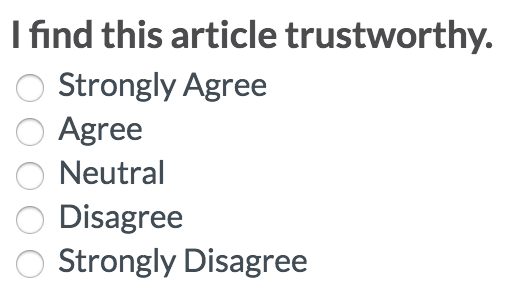
\includegraphics[width=.7\textwidth]{trust}  
%   \caption{Overall Trust Ratings
%     \label{fig:trust}}
% \end{figure}

\newpage
\begin{figure}[h!] 
\centering 
  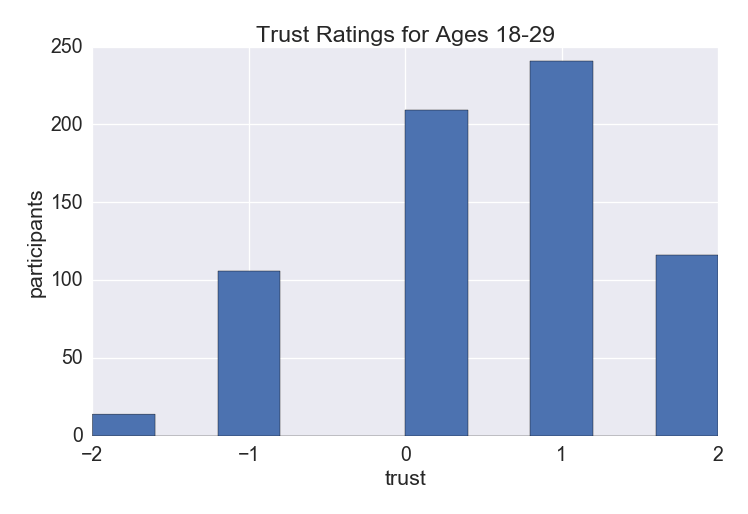
\includegraphics[width=0.8\textwidth]{trust_18-29} 
  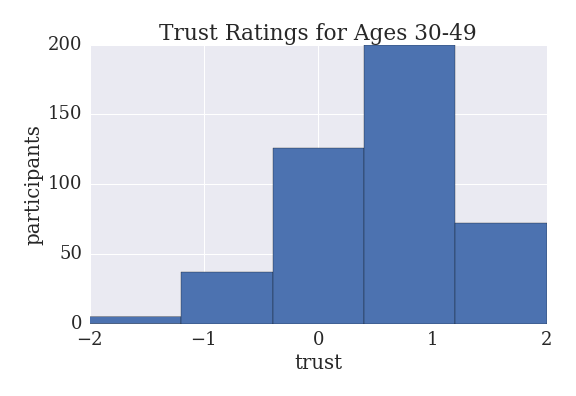
\includegraphics[width=0.8\textwidth]{trust_30-49} 
  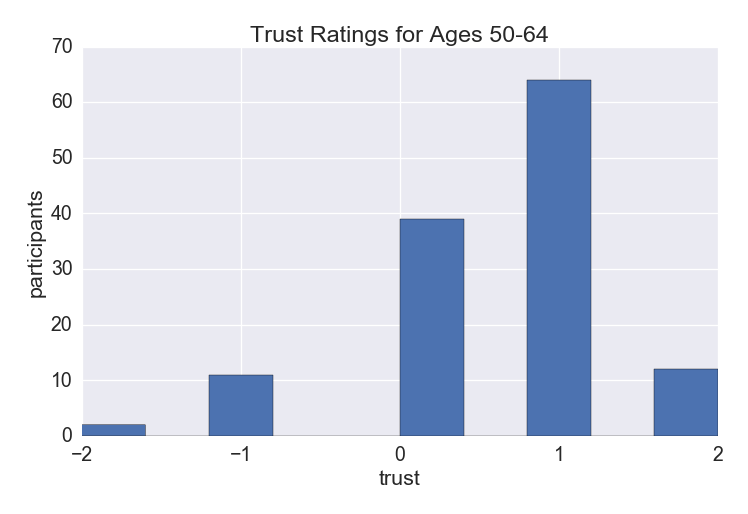
\includegraphics[width=0.8\textwidth]{trust_50-64} 
  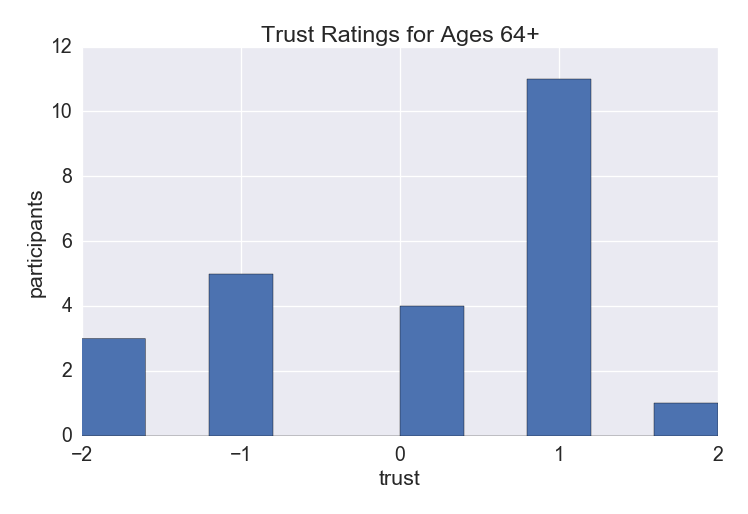
\includegraphics[width=0.8\textwidth]{trust_64+} 
  %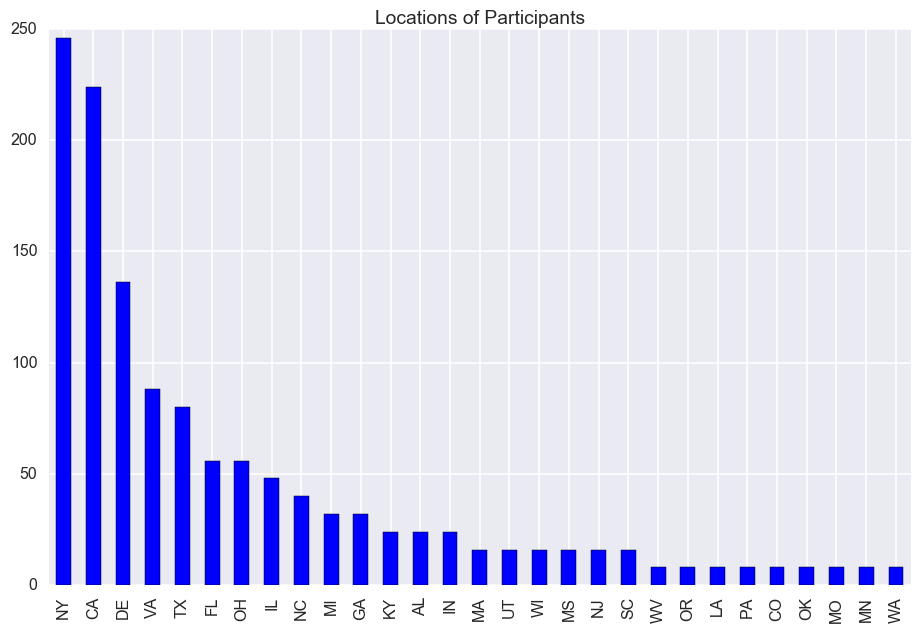
\includegraphics[width=0.32\textwidth]{location_study2} 
  \caption{Trust in Stories by Age Group
    \label{fig:trust-by-age}}
\end{figure}


% \begin{figure}[h!]  
% \centering 
%   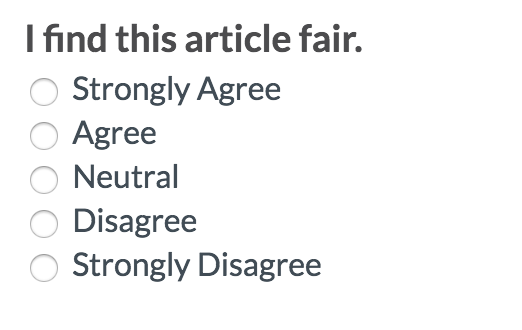
\includegraphics[width=.7\textwidth]{fair}  
%   \caption{Overall Fairness Ratings
%     \label{fig:fair}}
% \end{figure}

\newpage

% \begin{figure}[h!]  
% \centering  
%   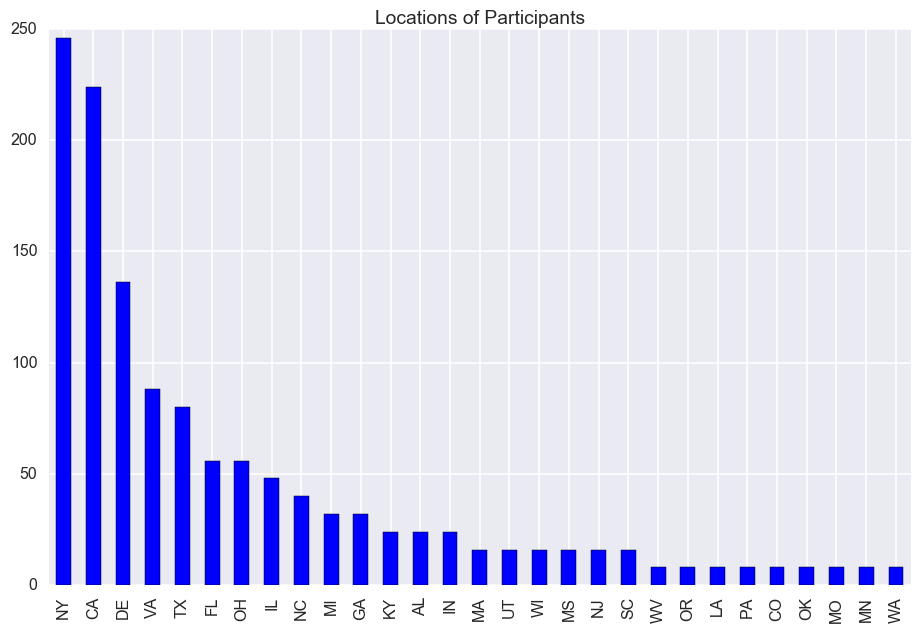
\includegraphics[width=0.9\textwidth]{location_study2} 
%   \caption{Locations of Participants
%     \label{fig:locations2}}
% \end{figure}

% \begin{figure}[h!]  
% \centering 
%   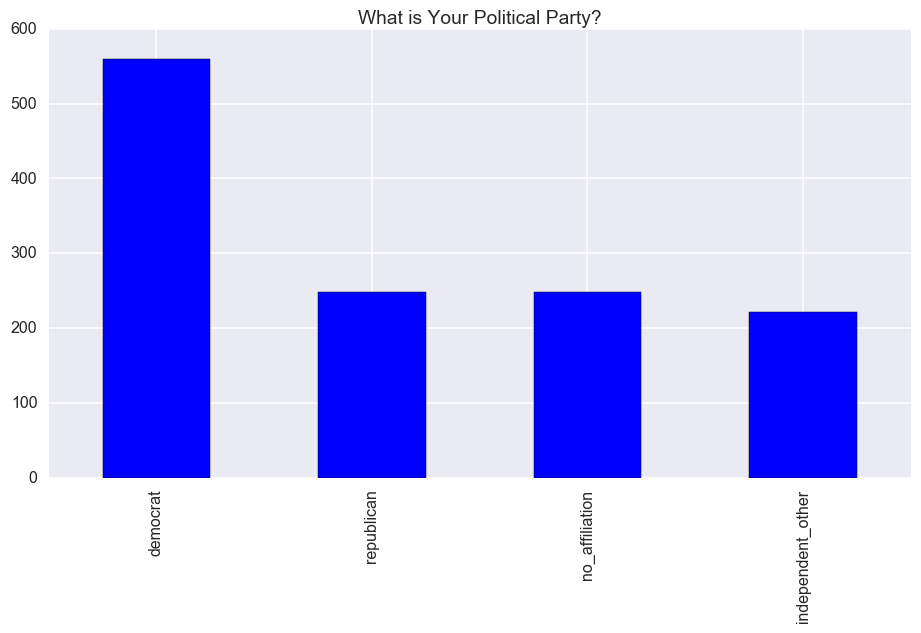
\includegraphics[width=.8\textwidth]{party_study2} 
%   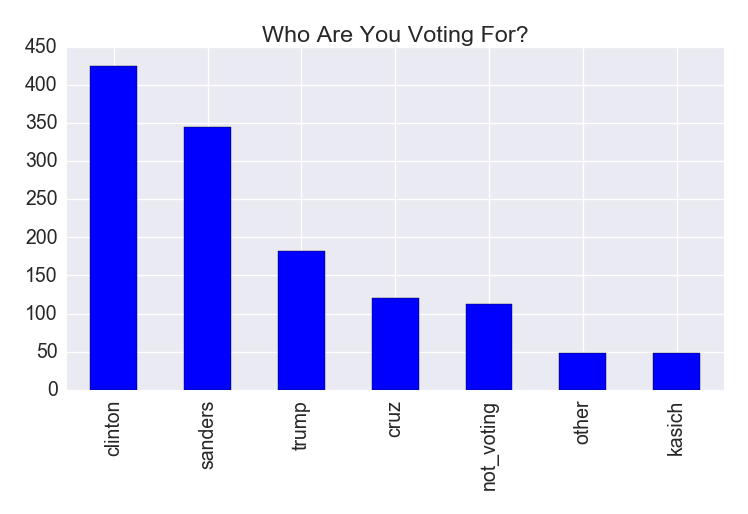
\includegraphics[width=.8\textwidth]{voting_for_study2} 
%   %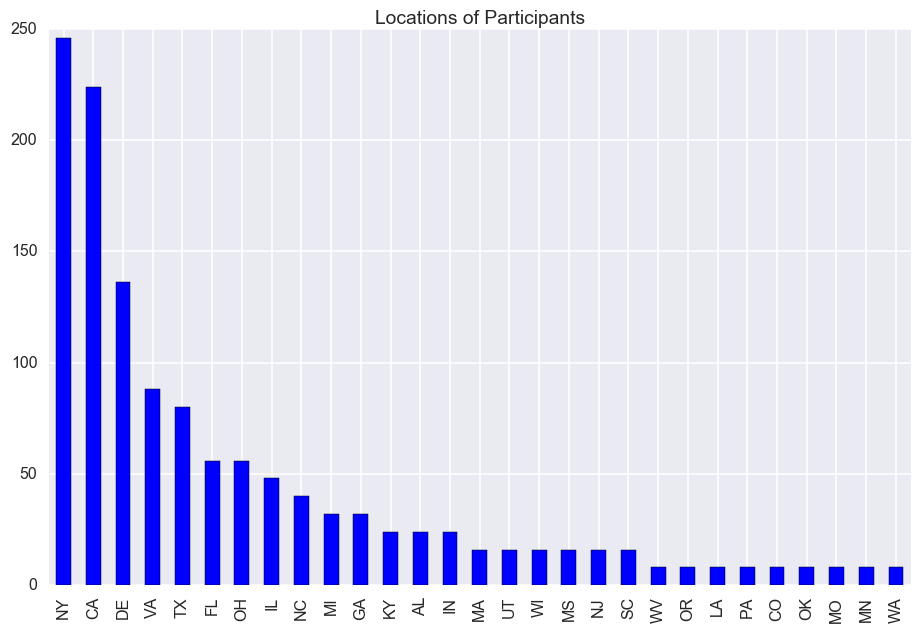
\includegraphics[width=0.32\textwidth]{location_study2} 
%   \caption{Political Affiliations of Participants
%     \label{fig:political2}}
% \end{figure}


% \begin{figure}[h!] 
% \label{fig:topics}
% \centering 
%   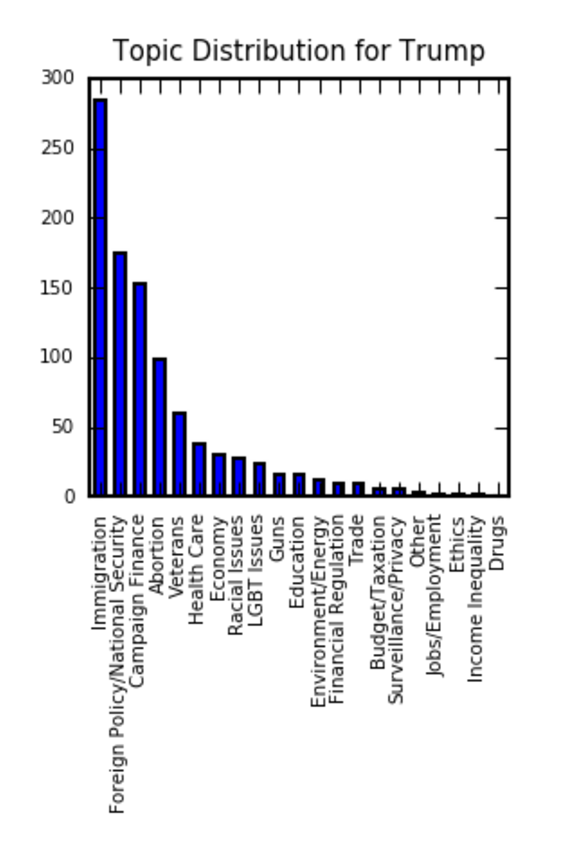
\includegraphics[width=0.45\textwidth]{trump_topics} 
%   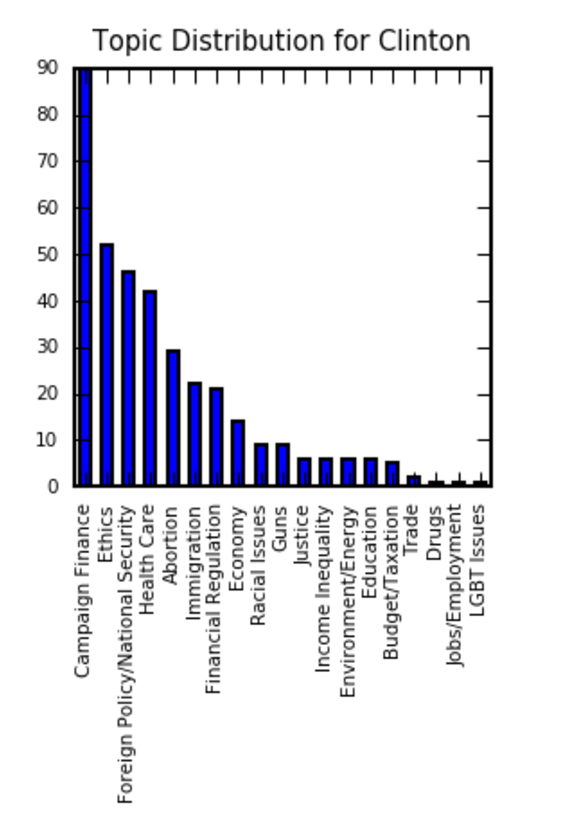
\includegraphics[width=0.45\textwidth]{clinton_topics} 
%   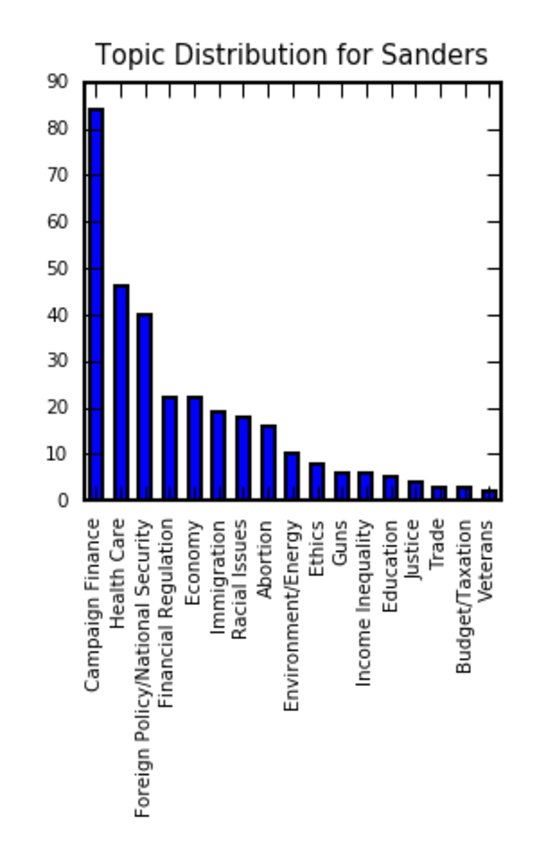
\includegraphics[width=0.45\textwidth]{sanders_topics} 
%   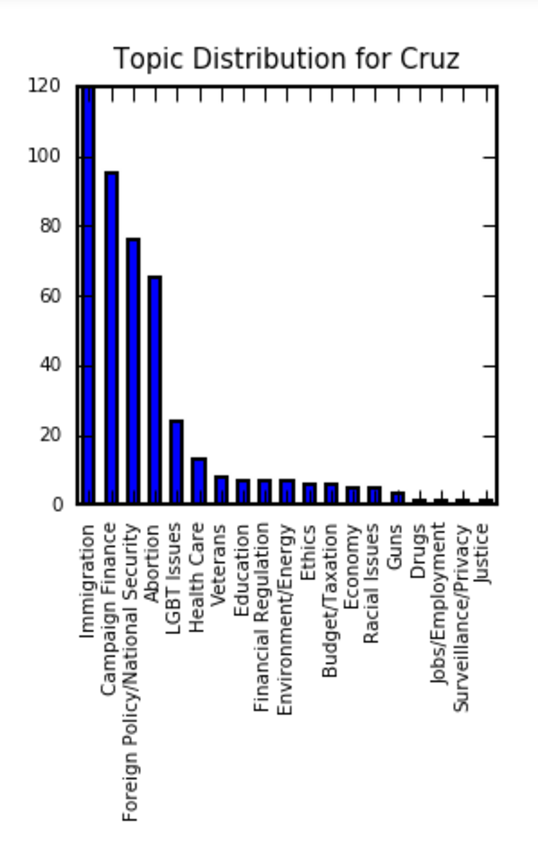
\includegraphics[width=0.45\textwidth]{cruz_topics} 
%   \caption{Topic Distributions for Candidates}
% \end{figure}
% \clearpage
% \newpage
%  
%% This defines the bibliography file (main.bib) and the bibliography style.
%% If you want to create a bibliography file by hand, change the contents of
%% this file to a `thebibliography' environment.  For more information 
%% see section 4.3 of the LaTeX manual.
\begin{singlespace}
\bibliography{main}
\bibliographystyle{plain}
\end{singlespace}

\end{document}

